This chapter describes the Recurrent Neural Network Grammar (RNNG), a probabilistic model of sentences with explicit phrase structure introduced by \citet{dyer2016rnng}. The model has a discriminative and generative formulation, but both are based on a shift-reduce transition system that builds trees in top-down order and define locally normalized probability distributions over action sequences. While the discriminative model is a constituency parser, the generative model is a joint model that can be evaluated both as constituency parser and as language model. The strength of both models lies in their unbouded history: at each step the model can condition on the entire derivation constructed thus far. This derivation is summarized by a syntax-dependent recurrent neural networks. This parametrization without independence assumptions, however, does preclude the use of exact inference---for example based on dynamic programming---but approximate inference based on greedy decoding and importance sampling provides tractable alternatives.

In this chapter:
\begin{itemize}
  \item We describe the discriminative and generative formulations of the RNNG in detail.
  \item We describe the approximate inference algorithms that allow the RNNG to be used as parser and as language model.
  \item We implement the models and reproduce the results of \citet{dyer2016rnng}.
\end{itemize}

\section{Model}
  The discriminative RNNG is a transition based parser that uses regular RNNs to summarize the actions in the history and the words on the buffer into vectors, and uses a special RNN with a syntax-dependent recurrence to obtain a vector representation of items on the the stack. The generative RNNG can be seen as a generative formulation of the RNNG that jointly models the words instead of merely conditioning on them. Alternatively, it can be seen as a structured model of language that predicts words together with their structure. From the parsing perspective, the generative RNNG simply dispenses with the buffer to instead predict the words. But as a model of sentences, it can best be understood as kind of structured RNN: it predicts words incrementally, but compresses and labels them recursively whenever they form a complete constituents. In this section we introduce both models, starting at their backbone: the transition system.

  \subsection{Transition sytem}
    Both RNNG models use a transition system crafted for top-down tree generation. The discriminative transition system has three actions:
    \begin{itemize}
      \item \open(X) opens a new nonterminal symbol X in the partially constructed tree.
      \item $\shift$ moves the topmost word $x$ from the buffer onto the stack.
      \item $\reduce$ closes the open constituent by composing the symbols in it into a single item representing the content of the subtree. This allows nodes with an arbitrary number of children.
    \end{itemize}
    How these actions work to build a tree is best illustrated with an example derivation.

    \begin{example}{(Discriminative transition system)}
      \label{ex:disc-states}
      The following table shows the consecutive states of the parser that produces the gold tree for input sentence \textit{The hungry cat sleeps}. Individual items are separated by the midline symbol.
      \begin{table}[!htbp]
\center
\footnotesize
  \begin{tabular}{r|l|l|l}
    & Stack & Buffer & Action  \\ \hline
    0 &  & \textit{The} \,$\mid$\, \textit{hungry}\,$\mid$\,\textit{cat}\,$\mid$\,\textit{meows}\,$\mid$\,. & \open(S) \\
    1 & (S & \textit{The}\,$\mid$\,\textit{hungry}\,$\mid$\,\textit{cat}\,$\mid$\,\textit{meows}\,$\mid$\,. & \open(NP) \\
    2 & (S\,$\mid$\,(NP  & \textit{The}\,$\mid$\,\textit{hungry}\,$\mid$\,\textit{cat}\,$\mid$\,\textit{meows}\,$\mid$\,. & \shift \\
    3 & (S\,$\mid$\,(NP\,$\mid$\,\textit{The} & \textit{hungry}\,$\mid$\,\textit{cat}\,$\mid$\,\textit{meows}\,$\mid$\,. & \shift \\
    4 & (S\,$\mid$\,(NP\,$\mid$\,\textit{The}\,$\mid$\,\textit{hungry} & \textit{cat}\,$\mid$\,\textit{meows}\,$\mid$\,. & \shift \\
    5 & (S\,$\mid$\,(NP\,$\mid$\,\textit{The}\,$\mid$\,\textit{hungry}\,$\mid$\,\textit{cat} & \textit{meows}\,$\mid$\,. & \reduce \\
    6 & (S\,$\mid$\,(NP\,\textit{The}\,\textit{hungry}\,\textit{cat}) & \textit{meows}\,$\mid$\,. & \open(VP) \\
    7 & (S\,$\mid$\,(NP\,\textit{The}\,\textit{hungry}\,\textit{cat})\,$\mid$\,(VP & \textit{meows}\,$\mid$\,. & \shift \\
    8 & (S\,$\mid$\,(NP\,\textit{The}\,\textit{hungry}\,\textit{cat})\,$\mid$\,(VP\,$\mid$\,\textit{meows} & . & \reduce \\
    9 & (S\,$\mid$\,(NP\,\textit{The}\,\textit{hungry}\,\textit{cat})\,$\mid$\,(VP\,\textit{meows}) & . & \shift \\
    10 & (S\,$\mid$\,(NP\,\textit{The}\,\textit{hungry}\,\textit{cat})\,$\mid$\,(VP \textit{meows})\,$\mid$\,. &  & \reduce \\
    11 & (S\,(NP\,\textit{The}\,\textit{hungry}\,\textit{cat})\,(VP\,\textit{meows})\,.) &  &  \\ \hline
  \end{tabular}
  \caption{Discriminative transition system. Example from \citet{dyer2016rnng}.}
% \caption{Discriminative transition sequence that parses an input sentence. Items are separated by the midline symbol $|$.}
% \label{tab:disc-trans}
\end{table}

    \end{example}

     The actions are constrained in order to only derive well-formed trees:
    \begin{itemize}
      \item $\shift$ can only be excecuted if there is at least one open nonterminal (all words must be under some nonterminal symbol).
      \item \open(X) requires there to be words left on the buffer (all constituents must eventually hold terminals).\footnote{Additionally, the number of open nonterminals can be at most some arbitrary number $n$, in practice 100. This constraint prevents the model from generating trees with arbitrarily long unary chains.}
      \item $\reduce$ requires there to be at least one terminal following the open nonterminal, and the topmost nonterminal can only be closed when the buffer is empty (all nodes must end under a single root node).
    \end{itemize}
    The generative transition system is derived from this system by replacing the $\shift$ action, which moves the word $x$ from the buffer into the open constituent on the stack, with an action that \textit{predicts} the word:
    \begin{itemize}
      \item $\gen(x)$ predicts that $x$ is the next word in the currently open constituent, and puts this word on the top of the stack.
    \end{itemize}
    The buffer is dispensed with and is replaced by a similar structure that records the sequence words predicted so far.

    \begin{example}{(Generative transition system)} Generating the sentence of example \ref{ex:disc-states} together with its tree.
      \begin{table}[h]
\center
\scriptsize
  \begin{tabular}{r|l|l|l}
    & Stack & Terminals & Action  \\ \hline
    0 &  &  & \open(S) \\
    1 & (S & & \open(NP) \\
    2 & (S\,|\,(NP  & & \gen(\textit{The}) \\
    3 & (S\,|\,(NP\,|\,\textit{The} & \textit{The} & \gen(\textit{hungry}) \\
    4 & (S\,|\,(NP\,|\,\textit{The}\,|\,\textit{hungry} & \textit{The}\,|\,\textit{hungry} & \gen(\textit{cat}) \\
    5 & (S\,|\,(NP\,|\,\textit{The}\,|\,\textit{hungry}\,|\,\textit{cat} & \textit{The}\,|\,\textit{hungry}\,|\,\textit{cat} & \reduce \\
    6 & (S\,|\,(NP\,\textit{The}\,\textit{hungry}\,\textit{cat}) & \textit{The}\,|\,\textit{hungry}\,|\,\textit{cat} & \open(VP) \\
    7 & (S\,|\,(NP\,\textit{The}\,\textit{hungry}\,\textit{cat})\,|\,(VP & \textit{The}\,|\,\textit{hungry}\,|\,\textit{cat} & \gen(\textit{meows}) \\
    8 & (S\,|\,(NP\,\textit{The}\,\textit{hungry}\,\textit{cat})\,|\,(VP\,|\,\textit{meows} & \textit{The}\,|\,\textit{hungry}\,|\,\textit{cat}\,|\,\textit{meows} & \reduce \\
    9 & (S\,|\,(NP\,\textit{The}\,\textit{hungry}\,\textit{cat})\,|\,(VP\,\textit{meows}) & \textit{The}\,|\,\textit{hungry}\,|\,\textit{cat}\,|\,\textit{meows} & \gen(\textit{.}) \\
    10 & (S\,|\,(NP\,\textit{The}\,\textit{hungry}\,\textit{cat})\,|\,(VP \textit{meows})\,|\,. & \textit{The}\,|\,\textit{hungry}\,|\,\textit{cat}\,|\,\textit{meows}\,|\,. & \reduce \\
    11 & (S\,(NP\,\textit{The}\,\textit{hungry}\,\textit{cat})\,(VP\,\textit{meows})\,.) & \textit{The}\,|\,\textit{hungry}\,|\,\textit{cat}\,|\,\textit{meows}\,|\,. &  \\ \hline
  \end{tabular}
% \caption{Generative transition sequences that \textit{generates} a sentence together with its constituency structures.}
% \label{tab:gen-trans}
\end{table}

    \end{example}

    With the transition system in place, we now move to describe how the RNNG defines a probability distribution over the sequeunces of transition actions.

  \subsection{Model}
    Fundamentally, the model is a probability distribution over transition action sequences $a = \langle a_1, \dots, a_T \rangle$ that generate trees $\y$.  Conditionally---given a sequence of words $\x$---in the discriminative model, and jointly---predicting the sequence $\x$---in the generative model. The model then defines a distribution over trees $\yieldx$ through the bijective transformation that maps transition sequences $a$ to trees $y$ and vice versa.\footnote{ Note that as a result of the transition system, the trees in the set $\yieldx$ are rather unconstrained: the trees can have any arity, and can contain arbitrarily long unary chains, depending on the maximum number of open nonterminals $n$ chosen.} Put simply, the model is thus defined as
    \begin{equation}
      \label{eq:naive-rnng-model}
      p( a ) = \prod_{t=1}^T p( a_t \mid a_{<t} ),
    \end{equation}
    where in the discriminative case $p( a ) = p( \y \mid \x )$ and in the generative model $p( a ) = p( \x, \y )$. The exact model however is slightly more complicated, a consequence of the difference between the discriminative and the generative actions and of practical concerns regarding the implementation. We will define the model more precisely. For this we need to introduce some things.

    First we define the set of discriminative actions as
    \begin{align}
      \discactions &= \{ \shift, \open, \reduce \},
    \end{align}
    and the set of generative actions as
    \begin{align}
      \genactions &= \{ \gen, \open, \reduce \}.
    \end{align}
    The finite set of nonterminals is denoted by $\Lambda$ and the finite alphabet of words by $\mathcal{X}$. For the discriminative model $a$ is sequence over $\discactions$, and in the generative model $a$ is a sequence over $\genactions$. In both cases $a$ is restricted to sequences that form a valid tree $\y$. The sequence of nonterminals $n = \langle n_1, \dots, n_K \rangle$ from $\Lambda^K$ is the sequence of nonterminal nodes obtained from a tree $\y$ by pre-order traversal, and we let a sentence $\x$ be an element of $\mathcal{X}^N$. Finally, we introduce two functions that map between sets of indices to indicate the number of times a particular action has been taken at each time step:
    \begin{align*}
      % \mu_a &: [ T ] \to [ K ]: t \mapsto \sum_{i=1}^{t-1} \indicator_{ \{ a_i \, = \, \open \} },
      % \mu_a &: \{ 1, \dots, T \} \to \{ 1, \dots, K \}: t \mapsto \sum_{i=1}^{t-1} \indicator_{ \{ a_i \, = \, \open \} },
      \mu_a &: \{ 1, \dots, T \} \to \{ 1, \dots, K \}: t \mapsto \sum_{i=1}^{t-1} \indicator(a_i = \open),
    \end{align*}
    and
    \begin{align*}
      % \nu_a &: [ T ] \to [ N ]: t \mapsto \sum_{i=1}^{t-1} \indicator_{ \{ a_i \, = \, \gen \} },
      % \nu_a &: \{ 1, \dots, T \} \to \{ 1, \dots, N \}: t \mapsto \sum_{i=1}^{t-1} \indicator_{ \{ a_i \, = \, \gen \} },
      \nu_a &: \{ 1, \dots, T \} \to \{ 1, \dots, N \}: t \mapsto \sum_{i=1}^{t-1} \indicator(a_i = \gen),
    \end{align*}
    but for brevity we drop the subscript $a$. We are now in the position to write down the exact models.

    % \begin{definition}{(Discriminative RNNG)}
    %   \label{def:disc-rnng}
    %   Let $a$ be a sequence over $\discactions$ of length $T$. Then the model for the discrminative RNNG is
    %   \begin{align*}
    %     p(\y \mid \x) = p(a \mid \x) = \prod_{t=1}^T P( a_t \mid \x, a_{<t}),
    %   \end{align*}
    %   where
    %   \begin{equation*}
    %     P( a_t \mid \x, a_{<t}) =
    %     \begin{cases}
    %       p( a_t \mid \x, a_{<t} ) p( n_{ \mu(t) } \mid \x, a_{<t} ) & \text{if } a_t = \open,  \\
    %       p( a_t \mid \x, a_{<t} ) & \text{otherwise.}  \\
    %     \end{cases}
    %   \end{equation*}
    %   Whenever the prediction is to open a new nonterminal the action probability factorizes as the product of two separate probabilities: the probability of the action itself, and the probability of the next upcoming label in $n$, which is indexed by $\mu(t)$.
    % \end{definition}

    \begin{definition}{(Discriminative RNNG)}
      \label{def:disc-rnng}
      Let $a$ be a sequence over $\discactions$ of length $T$, let $x$ be a sentence over $\mathcal{X}$ of length $N$, and let $n$ be the sequence on nonterminals over $\Lambda$ of length $K$ obtained from tree $y$. Then the model for the discrminative RNNG is
      \begin{align*}
        p(\y \mid \x)
          &\defeq p(a, n, \mid \x)  \\
          &= \prod_{t=1}^T
            p( a_t \mid u_t, x ) p(n_{ \mu(t) } \mid u_t, x )^{ \indicator(a_t = \open) },
      \end{align*}
      where $u_t \defeq (a_{<t}, n_{ <\mu(t) })$  is shorthand for the full history that is conditioned on at time $t$. Whenever the prediction is to open a new nonterminal the action probability factorizes as the product of two separate probabilities: the probability of the action itself, and the probability of the next upcoming label in $n$, which is indexed by $\mu(t)$.
    \end{definition}

    % \begin{definition}{(Generative RNNG)}
    %   \label{def:gen-rnng}
    %   Let $a$ be a sequence over $\genactions$ of length $T$. The model for the generative RNNG then is
    %   \begin{align*}
    %     p(\x, \y) = p(a) = \prod_{t=1}^T P( a_t \mid a_{<t}, n_{ <\mu(t) }, \x_{ <\nu(t) }),
    %   \end{align*}
    %   where
    %   \begin{equation*}
    %     P( a_t \mid a_{<t} ) =
    %     \begin{cases}
    %       p( a_t \mid a_{<t} ) p(n_{ \mu(t) } \mid a_{<t} ) & \text{if } a_t = \open,  \\
    %       p( a_t \mid a_{<t} ) p(x_{ \nu(t) } \mid a_{<t} ) & \text{if } a_t = \gen,  \\
    %       p( a_t \mid a_{<t} ) & \text{otherwise.}  \\
    %     \end{cases}
    %   \end{equation*}
    %   This corresponds with the discriminative model on the actions that they share. For the action that predicts the next word, the factorization is identical to that of the action that predicts the next nonterminal, with the difference that the next word in $x$ is instead indexed by $\nu(t)$.
    % \end{definition}

    \begin{definition}{(Generative RNNG)}
      \label{def:gen-rnng}
      Let $a$ be a sequence over $\genactions$ of length $T$, let $x$ be a sentence over $\mathcal{X}$ of length $N$, and let $n$ be the sequence on nonterminals over $\Lambda$ of length $K$ obtained from tree $y$. The model for the generative RNNG then is
      \begin{align*}
        p(\x, \y)
          &\defeq p(a, n, \x)  \\
          &= \prod_{t=1}^T
            p( a_t \mid u_t ) p(n_{ \mu(t) } \mid u_t)^{ \indicator(a_t = \open) } p(x_{ \nu(t) } \mid u_t)^{ \indicator(a_t = \gen) },
      \end{align*}
      where $u_t \defeq (a_{<t}, n_{ <\mu(t) }, \x_{ <\nu(t) })$ is shorthand for the full history that is conditioned on at time $t$. This corresponds with the discriminative model on the actions that they share. For the action that predicts the next word, the factorization is identical to that of the action that predicts the next nonterminal, with the difference that the next word in $x$ is instead indexed by $\nu(t)$.
    \end{definition}

    The probabilities in these products are computed by classifiers on a vector representation $\vecu_t$, which represents the parser configuration $u_t$ at time $t$. The probabilities are computed as
    \begin{align}
      p(a_t \mid u_{t})
        &\propto \exp \Big\{ [\ff_{\chi}( \vecu_t )]_{a_t}  \Big\}
    \end{align}
    and
    \begin{align}
      p(n_{\mu(t)} \mid u_{t}) \propto \exp \Big\{ [\ff_{\psi}( \vecu_t )]_{n_{\mu(t)}}  \Big\}
    \end{align}
    used by both models, and for the generative model alone
    \begin{align}
      p(x_{\nu(t)} \mid u_{t}) \propto \exp \Big\{ [\ff_{\xi}( \vecu_t )]_{x_{\nu(t)}}  \Big\},
      \label{eq:action-regression}
    \end{align}
    where we let $a_t$, $n_{\mu(t)}$, and $x_{\nu(t)}$ double as indices. We use different feedforward networks for the distributions, meaning that $\chi$, $\psi$, and $\xi$ are separate sets of parameters. The computation of the vector $\vecu_t$ is described in the next section.

    \begin{remark} We could have defined the actions as
      \begin{align*}
        \discactions &= \{ \reduce, \shift \} \cup \{ \open(n) \mid n \in \Lambda \},
      \end{align*}
      and
      \begin{align*}
        \genactions &= \{ \reduce \} \cup \{ \open(n) \mid n \in \Lambda \} \cup \{ \gen(x) \mid x \in \mathcal{X} \},
      \end{align*}
      and defined $p(a)$ as in \ref{eq:naive-rnng-model}. However, in the case of the generative model this is particularly inefficient from a computational perspective. Note that the set $\mathcal{X}$ is generally very large\footnote{On the order of tens or hundreds of thousands.}, and the normalization in \ref{eq:action-regression} requires a sum over all actions while a large number of the actions do not generate words. Besides, the presentation in definitions \ref{def:disc-rnng} and \ref{def:gen-rnng} is conceptually cleaner: first choose an action, then, if required, choose the details of that action. For these reasons we opt for the two-step prediction. For consistency we extend this modelling choice to the discriminative RNNG. And although it appears that \citet{dyer2016rnng} model the sequences according to \ref{eq:naive-rnng-model}, followup work takes our approach and models the actions of the generative RNNG as in definition \ref{def:gen-rnng} \citep{hale2018beam}.
    \end{remark}

\section{Parametrization}
  The transition probabilities are computed from the vector $\vecu_t$ that summarizes the parser's entire configuration history at time $t$. This vector is computed incrementally and in a syntax-dependent way. It is defined as the concatenation of three vectors, each summarizing one of the three datastructures separately:
  \begin{align*}
    \vecu_t = [\mathbf{s}_t; \mathbf{b}_t; \mathbf{h}_t].
  \end{align*}
  Here, $\mathbf{s}_t$ represents the stack, $\mathbf{b}_t$ represents the buffer, and $\mathbf{h}_t$ represents the history of actions.

  The vectors $\mathbf{b}_t$ and $\mathbf{h}_t$ are computed each with a regular RNN: the history vector is computed in the forward direction, and the buffer is encoded in the backward direction to provide a lookahead. The vector $\mathbf{s}_t$ represents the partially constructed tree that is on the stack, and its computation depends on this partial structure by using a structured RNN that encodes the tree in top-down order while recursively compressing constituents whenever they are completed.

  \subsection{Stack encoder}
    The stack RNN computes a representation based on incoming nonterminal and terminal symbols while these are respectively opened and shifted, as a regular RNN would, but rewrites this history whenever the constituent that they form is closed. Whenever a $\reduce$ action is predicted, the RNN rewinds its hidden state to before the constituent was opened; the items making up the constinuent are composed into a single vector by a composition function; and this composed vector is then fed into the rewound RNN as if the subtree were a single input. The closed constituent is now a single item represented by a single vector. Due to the nested nature of constituents this procedure recursively compresseses subtrees.

    \begin{example}{(Composition function)}
      Consider the state of the parser in example \ref{ex:disc-states} at step 5, when the stack contains the five items
      \begin{center}
        (S $\mid$ (NP $\mid$ \textit{The} $\mid$ \textit{hungry} $\mid$ \textit{cat}.
      \end{center}
      Each first represented by an embedding vector, and then encoded by an RNN in the regular way. A $\reduce$ action is now predicted: the items are popped from the stack until the first open bracket is popped, which in this example is the item that opens the NP bracket. This process also rewinds the RNN state to before the bracket was openend, which in this example brings the RNN back to its state at step 1. The composition now computes a vector representation for the four popped items, returning a single representation for the composed item
      \begin{center}
        (NP \textit{The} \textit{hungry} \textit{cat}).
      \end{center}
      The RNN is fed this reduced input, resulting in the encoding of stack at step 6, and finalizing the reduction step. This process is recursive: consider the reduction that takes the stack from the five items
      \begin{center}
        (S $\mid$ (NP $\mid$ \textit{The} $\mid$ (ADJP \textit{very} \textit{hungry}) $\mid$ \textit{cat}
      \end{center}
      to the two items
      \begin{center}
        (S $\mid$ (NP \textit{The} (ADJP \textit{very} \textit{hungry}) \textit{cat}).
      \end{center}
      The items in the constituent (ADJP \textit{very} \textit{hungry}) have already been composed into a single item, and now it takes part in the composition at a higher level.
    \end{example}

  \subsection{Composition function}
    Two kinds of functions have been proposed to for the composition described above: the original function based on a bidirectional RNN \citep{dyer2016rnng}, and a more elaborate one that additionally incorporates an attention mechanism \citep{kuncoro2017syntax}. Both methods encode the invidual items that make up the constituent with a bidirectional RNN, but where the simpler version merely concatenates the endpoint vectors, the attention based method computes a convex combination of all these vectors, weighted by predicted attention weights. \citet{kuncoro2017syntax} show that the models with the attention-based composition outperform the models with the simpler composition, and that the attention mechanism adds interpretability to the composition. For these reasons we only consider the attention-based composition.

    The attention-based composition is defined as follows. Let $\h_1, \dots, \h_m$ be the vector representations computed by a dedicated bidirectional LSTM for the $m$ words making up the constituent that is to be compressed, and let $\mathbf{n}$ be the learned embedding for the nonterminal category of that constituent. The attention weight $a_i$ for the $i$-th position is computed as the exponentiated bilinear product
    \begin{align*}
      a_i &\propto \exp \Big\{ \h_i^{\top} \mathbf{V} \, [\vecu_t ; \mathbf{n}] \Big\}
    \end{align*}
    between the vector representation $\h_i$ and the concatenation of current parser state representation $\vecu_t$ and nonterminal representation $\mathbf{n}$. The values $a_1, \dots, a_m$ are normalized to sum to 1, and the matrix $\mathbf{V}$ is part of the trainable parameters. The convex combination of the vectors $\h_i$ weighted by values $a_i$ gives the vector
    \begin{align*}
      \mathbf{m} = \sum_{i=1}^m a_i \mathbf{h}_i,
    \end{align*}
    which represents the words in the constituent, and the final representation of the constituent is the gated sum
    \begin{align*}
      \mathbf{c} = \mathbf{g} \circ \mathbf{n} + (1 - \mathbf{g}) \circ \mathbf{m}.
    \end{align*}
    of this vector and the vector $\mathbf{n}$ representing the nonterminal, weighted by a gating vector $\mathbf{g}$. The vector of gates $\mathbf{g}$ is computed by an affine transformation on $[ \mathbf{n}; \mathbf{m} ]$ followed by an elementwise application of the logistic function.\footnote{Our definition of $\mathbf{c}$ is slightly different from that of \citet{kuncoro2017syntax}: they use a vector representation $\mathbf{t}$ different from $\mathbf{n}$ in the above definition; we use $\mathbf{n}$ to compute both the attention weights and the final vector.} This final representation can weigh the contribution to the final representation of the words and their nonterminal category, depending on the context.

\section{Training}
  The discriminative and generative model are trained to maximize the log likelihood of a labeled dataset $\dataset$ of pairs $(\x, \y)$
  \begin{align*}
    \mathcal{L}(\theta) = \sum_{(\x, \y) \in \dataset} \log \ptheta (\y \mid \x),
  \end{align*}
  respectively
  \begin{align*}
    \mathcal{L}(\theta) = \sum_{(\x, \y) \in \dataset} \log \ptheta (\x, \y),
  \end{align*}
  by gradient-based optimization on the parameters $\theta$.

  % We perfom iterative parameter updates, optaining new parameters $\theta^{(t+1)}$ at timestept $t+1$ from parameters $\theta^{(t)}$ at timestep $t$ using the update rule
  % \begin{align*}
  %   \theta^{(t+1)} = \theta^{(t)} + \gamma^{(t)} \nabla_{\theta^{(t)}} \mathcal{L}( \theta^{(t)} ),
  % \end{align*}
  % where the value $\gamma^{(t)}$ is a time-indexed learning rate. We replace $\nabla_{\theta} \mathcal{L}(\theta)$ with an unbiased estimate
  % \begin{align*}
  %   \sum_{k=1}^{K} \nabla_{\theta} \log \ptheta (\x^{(k)}, \y^{(k)}),
  % \end{align*}
  % where pairs $(\x^{(k)}, \y^{(k)})$ are sampled uniformly from $\dataset$, which works because for uniformly random sampled pairs $(\x^{(s)}, \y^{(s)})$ from the dataset.
  % \begin{align*}
  %   \nabla_{\theta} \mathcal{L}(\theta)
  %     &\propto \expect [ \nabla_{\theta} \log \ptheta (\x^{(s)}, \y^{(s)}) ].
  % \end{align*}
  % We use minibatches for this estimates, making our optimization procedure stochastic. Under certain conditions on $\gamma^{(t)}$ this method is guaranteed to converge to a local optimum \citep{robbins1951stochastic}.


\section{Inference}
  The two formulations of the RNNG have complementary applications: both models can be used for parsing, but the generative model can additionally be used as a language model. How these problems can be solved is the topic of this section.

  \subsection{Discriminative model}
    Parsing a sentence $\x$ with the discriminative model corresponds to solving the following search problem of finding the maximum \textit{a posteriori} (MAP) tree
    \begin{align*}
      \hat{\y} = \argmax_{ \y \in \yieldx } \ptheta(\y \mid \x).
    \end{align*}
    Solving this exactly is intractable due to the parametrization of the model. At each timestep, the model conditions on the entire derivation history which excludes the use of dynamic programming to solve this efficiently. Instead we rely on an approximate search strategy. There are two common approaches for this: greedy decoding and beam search. We only focus on the first. Greedy decoding is precisely what it suggests: at each timestep we greedily select the best local decision
    \begin{align*}
      \hat{a}_t = \argmax_{a} \ptheta(a \mid \hat{a}_{< t}).
    \end{align*}
    The predicted parse is then the approximate MAP tree $\y^* = \text{yield}(\hat{a})$, which is the tree constructed from the sequence $\hat{a} = \langle \hat{a}_1, \dots, \hat{a}_m \rangle$.

  \subsection{Generative model}
    Given a trained generative model $\ptheta$ we are interested in solving the following two problems: parsing a sentence $\x$
    \begin{align*}
      \hat{\y} = \argmax_{ \y \in \yieldx } \ptheta(\x, \y),
    \end{align*}
    and computing its marginal probability
    \begin{align*}
      p(\x) = \sum_{ \y \in \yieldx } \ptheta(\x, \y).
    \end{align*}
    Either inference problem is intractable. Computing the marginal requires a sum over all possible action sequences, and the lack of conditional independence between actions inhibits any approach based on dynamic programming. Parsing would similarly require exhaustive enumeration of all trees. Luckily, both problems can be effectively approximated with the same approximate inference method: importance sampling using a conditional proposal distribution $\qlambda(\y \mid \x)$ \citep{dyer2016rnng}.

    \paragraph{Approximate marginalization}
      The proposal distribution allows us to rewrite the marginal probability of a sentence as an expectation under this distribution:
      \begin{align*}
        p (\x)
          &= \sum_{\y  \in \mathcal{Y}(\x)} \ptheta(\x, \y) \\
          &= \sum_{\y  \in \mathcal{Y}(\x)} \qlambda(\y \mid \x) \frac{\ptheta(\x,\y )}{\qlambda(\y \mid \x)} \\
          &= \expect_{q} \bigg[\frac{\ptheta(\x,\y )}{\qlambda(\y \mid  \x)} \bigg] \\
      \end{align*}
      This expectation can be approximated with a Monte Carlo estimate
      \begin{align}
        \expect_{q} \bigg[\frac{\ptheta(\x, \y)}{\qlambda(\y \mid \x)} \bigg]
          &\approx \frac{1}{K}\sum_{k=1}^K  \frac{\ptheta( \x, \y^{(k)} )}{\qlambda(\y^{(k)} \mid \x)},
      \end{align}
      using proposal samples $\y^{(k)}$ sampled from the proposal model $\qlambda$ conditioning on $\x$.

    \paragraph{Approximate MAP tree}
      To approximate the MAP tree $\hat{\y}$ we use the same set of proposal samples as above, and choose the tree $\y$ from the proposal samples that has the highest probability probability under the joint model $\ptheta( \y, \x)$. We thus effectively use the generative model to rerank proposals from the discriminative model.

      The rationale behind this is as follows. We want to obtain trees $\y$ for which the true posterior $\ptheta(\y \mid \x) = \ptheta( \x, \y ) /\ptheta(\x)$ is high. If $\qlambda$ is similar to this true posterior, it will tend to produce samples $\y$ for which $\ptheta(\y \mid \x)$ is also high. The tree $\y$ that is highest under $\ptheta( \x, \y )$ will then also be highest under $ \ptheta( \y \mid \x )$ because
      \begin{align*}
        \argmax_y \ptheta( \y \mid \x ) = \argmax_y \ptheta(\x, \y),
      \end{align*}
      which is precisely what we wanted. For this approximation it is thus beneficial for the proposal model $\qlambda(\y \mid \x)$ to be `close to' the true posterior $\ptheta(\y \mid \x)$. \footnote{The notion of `close to' is made precise in variational inference as the KL divergence between $\qlambda$ and the true posterior in a setup similar to this. About this more in chapter \ref{05-semisupervised}.}

    \paragraph{Proposal distribution}
      The proposal distribution must have a support that covers that of the joint model. This corresponds to the property that for all $\x$ and $\y \in \yieldx$
      \begin{equation*}
        p(\x, \y) > 0 \Rightarrow q( \y \mid \x ) > 0.
      \end{equation*}
      We additionally want that the samples can be obtained efficiently, and that their conditional probability can be computed. All these requirements are met by the discriminative RNNG: samples can be obtained by ancestral sampling over the transition sequences, and their probability is given by the product of probabilities of these transition actions. \citet{dyer2016rnng} use this as their proposal, and in this chapter we will follow their example. In principle, any discriminatively trained parser that meets these requirements can be used, but as we argued in the previous paragraph: the closer to the true posterior $\ptheta(\y \mid \x)$ the better.

\section{Experiments}
  This section reports the results of the experiments performed with our own implementation of the RNNG. We train the discriminative and generative model on the Penn Treebank with the same hyperparameters as \citet{dyer2016rnng}, and compare our results to conclude the correctness of our implementation. We then investigate how the approximate marginalization depends on two parameters: the number of samples, and the temperature used to scale the distribution of the proposal model. For the general training setup and details about data and optimization we refer the reader to appendix \ref{A2-implementation}.

  \subsection{Setup}
    We use the same hyperparameters as \citep{dyer2016rnng}. For both models the embeddings are of dimension 100, and the LSTMs have 2 layers. The LSTMs have dimension 128 in the discriminative model and 256 in the generative model, and the dimension of the feedforward networks that compute the action distributions are the same as the LSTMs. We use weight decay of $10^{-6}$, and apply dropout to all layers including the recurrent connections\footnote{Also called \textit{variational dropout} \citep{gal2016theoretically}, which is implemented by default in Dynet \citep{neubig2017dynet}.} using a dropout ratio of 0.2 in the discriminative model and 0.3 in the generative model. Given the above dimensions, the total number of trainable parameters is approximately 0.8M for the discriminative model and 9.6M for the generative model (the exact numbers are given in table \ref{tab:num-params}).

    Our discriminative model does not use tags, which contrasts with \citet{dyer2016rnng} who use tags predicted by an external tagger. This decision was made with the application of the RNNG as language model in mind, in which case tags are not available, but this choice will affect the parsing accuracy of the discriminative model. For a more elaborate justification of this choice we refer the reader to section \ref{sec:impl-embedding} of the implementation appendix \ref{A2-implementation}.

    % \begin{itemize}
    %   \item Training on a single CPU takes ... per epoch for the discriminative model, and ... for the generative model.
    %   \item The models take ... days to converge.
    % \end{itemize}

  \subsection{Results}
    We train 10 separate models from different random seeds.\footnote{The random seeds control both the random initialization of the model parameters as well as the order in which we pass through the training data.} We report mean and standard deviation to give a sense of the variability of the accuracy, as well as the value of the model with the best development performance. Model selection is based on development F1 for the discriminative model, and based on development perplexity for the generative model. For inference with the generative model we follow \citet{dyer2016rnng} and sample 100 trees from our best discriminative model. The samples are obtained by ancestral sampling on the action sequeunces, and we flatten this ditribution by raising each action distribution to the power $\alpha = 0.8$ and renormalizing it.

    The parsing F1 of the discriminative model are shown in table \ref{tab:disc-fscores}, and the results of the generative model are shown in tables \ref{tab:gen-fscores} (F1) and \ref{tab:gen-perplexities} (perplexity). The value between brackets is the value based on model selection.

    \begin{table}[h]
\center
  \begin{tabular}{l|c|c}
        & Ours & \citet{dyer2016rnng}  \\ \hline
    F1  & $88.47 \pm	0.17 \quad (88.58)$ & -- \quad (91.7)
  \end{tabular}
  \caption{F1 scores for the discriminative RNNG.}
  \label{tab:disc-fscores}
\end{table}


% The first value shows the mean and standard deviation over 10 models trained from different random seeds. The second value (in brackets) shows the score of the single model selected by development score. Note that our rnng is trained without tags.


    \begin{table}[h]
\center
\footnotesize
  \begin{tabular}{l|c|c|c}
      Proposals & Our RNNG & CRF & \citet{dyer2016rnng} &  \\ \hline
      Ours  & $91.07 \pm	0.1 \quad (91.12)$  &  $91.02 \pm 0.05 \quad (91.04)$ &  $93.32 \pm 0.1 \quad (93.32)$  \\
      \citet{dyer2016rnng}  & -- & -- & -- \quad (93.3)
  \end{tabular}
  \caption{F1 scores for the generative RNNG, for different proposal samples. The first column is with proposals from our best discriminative RNNG and the second column is with the proposals used by \citet{dyer2016rnng}, availlable at \url{https://github.com/clab/rnng}.}
  \label{tab:gen-fscores}
\end{table}


    \begin{table}[h]
\center
\footnotesize
  \begin{tabular}{l|c|c}
        & Our samples & \citet{dyer2016rnng} samples \\ \hline
      Ours & $108.76 \pm	1.52 \quad (107.43)$ & $107.80 \pm 1.59 \quad (106.45)$  \\
      \citet{dyer2016rnng}  & -- & -- \quad (105.2)  \\
      \citet{kuncoro2017syntax} & -- & -- \quad (100.9)
  \end{tabular}
  \caption{Perplexity of the generative RNNG for different proposal models.}
  \label{tab:gen-perplexities}
\end{table}


    The accuracy of our discriminative model is below that of \citet{dyer2016rnng}, a gap that we think can reasonably be attributed to the absence of tag information in our implementation. This gap in F1 is carried through in a lesser degree to the generative model, resulting in a lower F1 than reported by \citet{dyer2016rnng} when using our own samples. The reranking by the generative models still finds better trees than the greedy decoding of the discriminative model, as evidenced by the higher F1 score, and when we evaluate with the proposal samples used in the original work we find that the F1 agrees perfectly with that of \citet{dyer2016rnng} and is on par with the results reported in \citet{kuncoro2017syntax}.\footnote{The proposal samples used by \citet{dyer2016rnng} are availlable at \url{https://github.com/clab/rnng}.}. The difference in perplexity performance is less pronounced, and with our own samples we manage to get close to the perplexity published in \citet{dyer2016rnng}. The perplexity does lag behind the results reported in \citet{kuncoro2017syntax}, which are the results obtained with the attention-based composition function.

  \subsection{Analysis}
    We now take a closer look at the approximate inference of the RNNG. The temperature $\alpha$ affects the proposal model and this, together with the number of samples, affects the approximate inference of the generative model. The temperature is used to flatten the proposal distribution to more evenly cover the support of the joint model, with the rationale of thus being closer to the true posterior;\footnote{After all, the proposal model was trained on a maximum likelihook objective, and we can thus expect it to be too peaked.} the number of samples is used to increase the accuracy of our unbiased MC estimate. The number of samples should particularly garner our attention: the approximate marginalization is compuationally expensive, requiring at least as many forward computations as there are unique samples.\footnote{For efficiency we already partition the samples into groups of identical samples, where for each group we need to compute just ones and scale by the size of the group.} The less samples we can get away with the better. To see how these values affect the generative RNNG in practice we perform two experiments: first we evaluate the RNNG with increasing number of samples, obtained with and without annealing; then we use these same samples to estimate the conditional entropy of the proposal models.

    For the first experiment we evaluate the generative RNNG as in the above setting, while varying the number of samples, and the temperature $\alpha$: we let the number of samples be in $\{ 10, 25, 50, 75, 100 \}$ and let $\alpha$ be in $\{ 0.8, 1 \}$.\footnote{When $\alpha=1$, the distribution is left unchanched.}. To quantify the variability of the proposal model in this we repeat the experiment 10 times. Figure \ref{fig:samples-fscores} shows the results of this experiment for the parsing F1, and \ref{fig:samples-perplexities} shows the results for the perplexity. The F1 of the generative model increases with the number of samples, but clearly converges at around 100 samples; the difference between 10 and 100 samples is about 1 F1 on average. This appears to tell us that the generative model finds the better trees at the tails of the proposal distribution---the trees that are only observed, on expectation, given enough samples. There is little difference between the different temperature values when using many samples, but when few samples are used the proposal model that is left unchanged performs best. In the case of perplexity we can see a consistent difference between the values of $\alpha$, always favoring the proposal model where $\alpha = 0.8$. A striking feature that can be observed in the plot is that the perplexity estimates lie in small regions that decrease with increasing number of samples. The estimate is in fact an \textit{upper bound} on the perplexity, a result of our estimator, the definition of perplexity, and Jensen's inequality.\footnote{We compute $p(x)$ as an expectation $\expect [p(x,y)]$, and because $\log \expect [p(x,y)] \leq \expect [\log p(x,y)]$ by Jensen's inequality we find for our perplexity estimate that $\exp \{ - \frac{1}{m} \log \expect [p(x,y)] \} \geq \exp \{ - \frac{1}{m} \expect [\log p(x,y)] \} $.} Each of the independent estimates vary litle between each other, but the gap between 10 and 100 samples is a significant 10 nats in perplexity, on avergare. It moreover appears from the trend of the curve that 100 samples is not yet enough to close the bound, and that more samples would still further lower the perplexity---an unfortunate finding given our concerns about computational efficiency.

    \begin{figure}[h]
      \center
    	\includegraphics[width=0.9\textwidth]{sample-experiment/fscore/disc_temp.pdf}
      \caption{F1 estimated with increasing number of samples, with and without annealed distributions, for 10 independent repetitions. Horizontal lines show values of individual outcomes.}
      \label{fig:samples-fscores}
    \end{figure}

    \newgeometry{}  % enables full page view
    \begin{figure}[ht]
      \center
    	\includegraphics[width=0.9\textwidth]{sample-experiment/ppl/disc_temp.pdf}
      \caption{Perplexity estimated with increasing number of samples, with and without annealed distributions, for 10 independent repetitions. Horizontal lines show values of individual outcomes.}
      \label{fig:samples-perplexities}

    	\includegraphics[width=0.4\textwidth]{sample-experiment/entropy/disc_temp.pdf}
      \caption{Conditional entropy estimated with increasing number of samples, with and without annealed distributions, for 10 independent repetitions. Horizontal lines show values of individual outcomes.}
      \label{fig:samples-entropy}
    \end{figure}
    \restoregeometry

    We move to the second experiment. To quantify the uncertainty in the discriminative proposal model we compute the conditional entropy. The conditional entropy of $Y$ given $X$ is defined as
    \begin{align*}
      \entropy(Y \mid X) &= \sum_{x \in \mathcal{X}} p(x) \entropy(Y \mid X = x),
    \end{align*}
    where
    \begin{align*}
      \entropy(Y \mid X = x)
        &= - \sum_{y \in \mathcal{Y}} p(y \mid x) \log p(y \mid x).
    \end{align*}
    In our case, the distribution $p$ is given by the discriminative RNNG. Because for this model the sum over $\mathcal{Y}$ cannot be computed efficiently we estimate it with a Monte Carlo estimate as
    \begin{align*}
      \entropy(Y \mid X = x)
        &= - \expect [ \log p(Y \mid X = x)]  \\
        &\approx - \frac{1}{K} \sum_{k=1}^K \log p(y^{(k)} \mid x),
    \end{align*}
    for which we can use the same samples $y^{(k)}$ drawn from $p(Y \mid X = x)$ as in the above experiments. To estimate the sum over $\mathcal{X}$ we can use the test set $\dataset$ that, which we consider a large sample from the data distribution $p(x)$:
    \begin{align*}
      \entropy(Y \mid X)
        &\approx \frac{1}{\lvert \dataset \rvert} \sum_{ (x, y) \in \dataset } \entropy(Y \mid X = x).
    \end{align*}
    What this means effectively is that we compute the average negative log-likelihood over all samples, for all sentences in the test set. We repeat this for each of the 10 sets of samples, for the same increasing number of samples. The results are show in figure \ref{fig:samples-entropy}. The results are as expected: the estimate converges as the number of samples increases, and the entropy of the proposal model flattened with $\alpha = 0.8$ is much higher than that of the original.


\section{Related work}

  % \subsection{Generative parsing}
    Most directly related to the RNNG is the work on generative dependency parsing \citep{titov2007generative,buys2015bayesian,buys2015generative,buys2018exact} and the work on language modelling via top-down generative parsing models in \citet{roark2001probabilistic}.

  % \subsection{Syntax}
    It has been investigated what RNNGs learn about syntax beyond their supervision. \citet{kuncoro2017syntax} show that the attention mechanism in the composition function learns a type of `soft' head-rules\footnote{A head is the lexical item in a phrase that determines the syntactic category of that phrase, \cf the background.}, in which most of the attention weight is put on the item that linguist consider the synactic head of such constituents. Another finding shows that when trained on unlabeledd trees, the RNNG learns representations for constituents that cluster according to their withheld gold label. Additionally, it has been found that RNNGs are much better at a long-distance subject-verb agreement task than LSTMS \citep{linzen2016syntax,kuncoro2018learn}, which advantage they owe to the composition function that by repeatedly compressing intervening structure decreases the distance between the two words at stake.

  % \subsection{Cognition}
    It appears also that RNNGs can tell us something about our brains: psycholinguistic research has shown that top-down parsing is a cognitively plausible parsing strategy \citep{brennan2016abstract}, and recently, RNNGs have been shown to be particularly good statistical predictors for human sentence comprehension \citep{hale2018beam}. In this experiment, the sequential word-probabilities derived from a generative RNNG\footnote{Obtained by using `word-synchronous beam-search' \citep{stern2017beam}.} provide a per-word complexity metric that predict human reading difficulty well. Much better at least than predictions from the word probabilities obtained from a purely sequential RNN language model.
